%Projects
%--------
%
%An essential part of this course are the take-home projects.
%
%Instructions for the take-home exams:
%
% Reports can be done individually or in groups of two. However, reasonably open
% discussions of the assignments with other students in this course are
% acceptable, but must be acknowledged in the report. The reports should consist
% of two to five pages plus supplementary graphs, tables, program listings, etc.,
% and should be organized as follows:
%
% Introduction and Problem Background. Briefly describe the general problem you
% want to solve and why a numerical or computational solution (as opposed to an
% exclusively analytical solution) is required.
%
% Numerical Considerations. Briefly discuss the specific methods, software or
% algorithms you selected for this problem. Mention any specific features of
% MATLAB you exploited.
%
% Results.  Include a concise tabular or graphical presentation of the results.
% Every table and figure should have a caption and a title, and the axes of every
% plot should be clearly marked, so that the reader can understand the figures or
% plots without referring to the main text. All codes should be clearly
% documented, especially input and output parameters, if any, and a description
% of what the code does.
%
% Analysis. Include a solid discussion and analysis of the results presented.
% The discussion should address any difficulties you encountered, appropriate
% measures of performance (such as errors and computer time) and the apparent
% sources of error you observed.
%
% Lessons Learned. Elaborate a critical evaluation of the software you used. Make
% a list of the specific things you  learned by working out the assignment, both
% theoretical and practical issues.
%
% Acknowledgements. Mention discussions with other students or teachers, software
% downloaded from the web or  copied from a book, and any other relevant
% information you find fit to disclose.
%
% The grade you obtain will reflect whether or not you have correctly and
% efficiently solved the problem, and whether or not you adequately address the
% relevant theoretical and practical issues. A grade of 8-12 indicates work that
% is acceptable, contains only minor errors, but is otherwise unexceptional. A
% grade of 13-15 indicates work that is correct, especially efficient and well
% documented, addresses all the points mentioned above, and contains unusually
% clear outputs and a serious and thorough analysis of those outputs.
%
% The report may be written in Swedish or English. Include name(s), ID number(s)
% and e-mail(s).
%
% Please hand in the report on paper (not via e-mail) at a lecture or seminar, or
% else place it in the box marked FMNF05 at the bottom of the shelf located at
% the entrance of the right-hand side corridor (MH, ground floor). The first
% report will be collected at 12:00 on Feb 2, 2018. The second project will be
% collected at 12:00 on Feb 23, 2018. Any report handed in or placed in the box
% after this time will not be accepted.

\documentclass{article}

\usepackage{rotating}
\usepackage[utf8]{inputenc}
\usepackage[T1]{fontenc}
\usepackage{gensymb}
\usepackage{amsmath}
\usepackage{graphicx}
\usepackage{verbatim}

\setlength\parindent{0pt}

\newcommand{\T}[2]{\textbf{Task #1} -- #2:\\}

\begin{document}

\begin{center}
  {\small FMNF05 - Computational Project 2} \\
  {\Large\textbf{Designing a car using tension splines}} \\
  %\vspace{0.4cm}
  \today\\
  %\vspace{0.2cm}
  Stefan Eng \texttt{<atn08sen@student.lu.se>} \\
  \vspace{0.2cm}
  {\Large ---}
  \vspace{-0.8cm}
\end{center}

\section*{Introduction}

  The problem consists of exploring the properties of \textit{tension splines}
  in order to use these to approximate the curvature of a car as close as possible.

  \begin{figure}[!ht]
    \center
    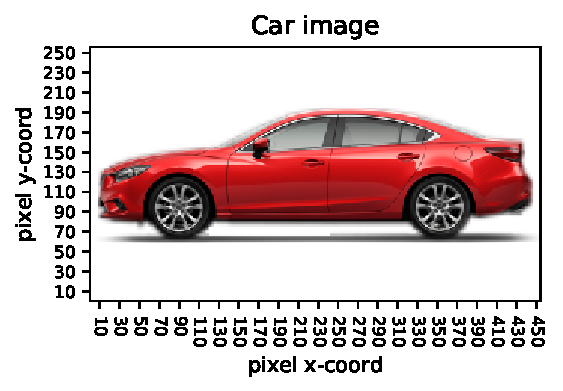
\includegraphics{figs/p2-car.pdf}
    \caption{Chosen car picture for silhouette tracing.}
  \end{figure}

  Since a function that reproduces the silhouette has not been provided, the
  function will have to approximated by choosing a number of appropriate knots
  by hand and then fitting a curve to them by numerical means.

\section*{Numerical Considerations}

  This project-solution utilizes \textit{Python} in combination with the
  modules \textit{numpy}, for numerical computations, and \textit{matplotlib}
  for producing plots and figures. \\

  Information on how to derive the coefficients for cubic splines, as well as
  how to plot the splines themselves has been gathered from chapter 3.4 in
  \textit{Numerical Analysis} by Timothy Sauer.  The same methodology is then
  re-used for deriving coefficients and plotting when switching to tension
  splines, modified slightly in order to fit the additional instructions
  provided by the project.

\section*{Result}

%\T{1}{Silhouette fitting - Cubic spline}

  Initial trace of upper curvature using a cubic spline, table of points
  available in appendix.

  \begin{figure}[!h]
    \center
    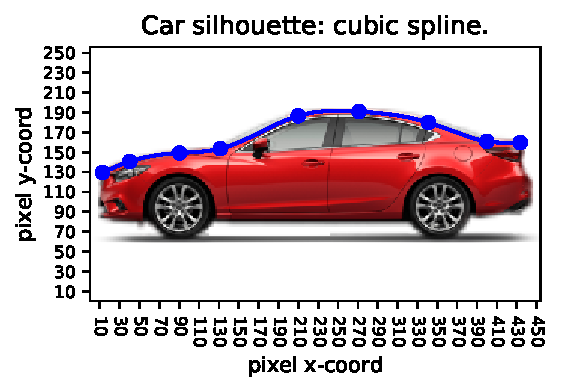
\includegraphics{figs/p2-car-grid-cubic.pdf}
    \caption{Upper curvature fit with cubic spline.}
  \end{figure}

  Tracing the same upper curvature using four three-point tension splines.

  \begin{figure}[!h]
    \center
    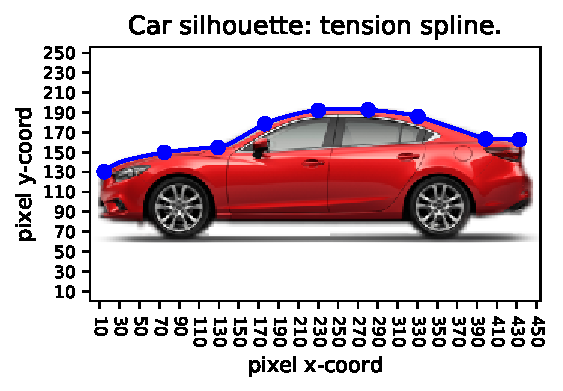
\includegraphics{figs/p2-car-tension-splines.pdf}
    \caption{Upper curvature fit with tension splines.}
  \end{figure}

\newpage

  This section contains tension splines rendered for different tension values
  and different beginning- and end-conditions.

  \begin{figure}[!h]
    \center
    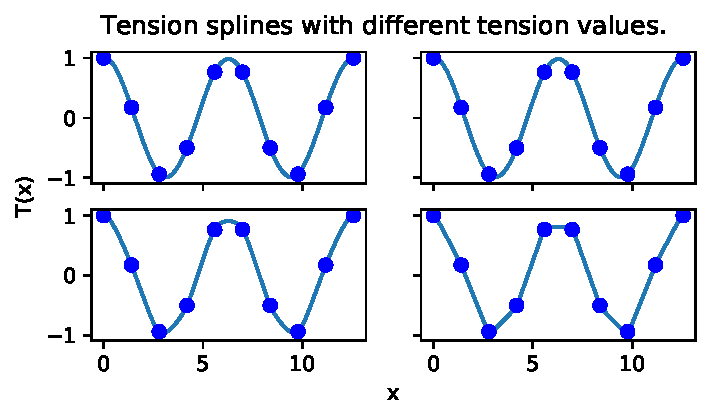
\includegraphics{figs/p2-fit-10-points.pdf}
    \caption{Tension splines interpolating 10 points along $f(x) =
    \mathrm{cos}(x)$, $x \in [0,4\pi]$ with tensions values $\tau = \{0.01,
    0.1, 3.0, 10.0\}$}
  \end{figure}

  \begin{figure}[!h]
    \center
    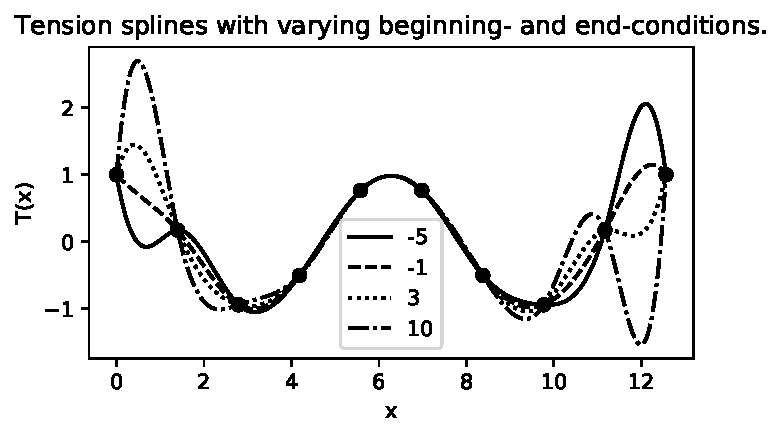
\includegraphics{figs/p2-fit-10-points-y0.pdf}
    \caption{Tension splines interpolating $\mathrm{cos}(x)$, same interval as
    previous figure, with different start- and end-conditions; $y'_0 = y'_n$
    and $\tau = 0.01$.}
  \end{figure}

  And lastly, additional curvature approximations for the cars under-side and
  general window outline, larger image available in appendix.

  \begin{figure}[!h]
    \center
    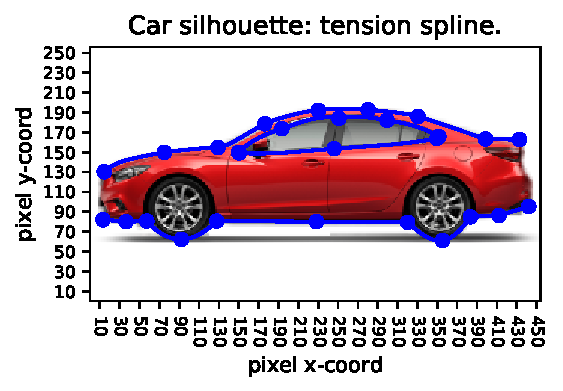
\includegraphics{figs/p2-car-tension-splines-extra.pdf}
    \caption{Additional curvature fit with tension splines.}
  \end{figure}

\section*{Analysis}

  \subsection*{Boundary analysis for 3'rd property of tension spline}

%\T{2}{Boundary analysis for $\tau$}

  The third property of the tension-spline is defined as:

  \begin{center}
  $
    T''''(x) - \tau^2 \cdot T''(x) = 0 \iff
    T''''(x) = \tau^2 \cdot T''(x)
  $
  \end{center}

  for each $ x \in [x_{i-1},x_i]$. Given $ \tau = 0 $, $T''''(x)$ becomes zero,
  indicating that the function will not behave as a polynomial with higher
  degree than three, i.e. a cubic spline. Worth noting; $\tau$ can come
  arbitrarily close to zero, but can't equal to zero as it appears in the
  denominator of expressions used in this project, both on its own and as the
  parameter to functions that become zero when $\tau$ is zero. \\

  If $\tau \rightarrow \infty$, $T''''(x) \rightarrow -\infty/\infty$,
  depending on the sign of $T''(x)$.
  The function will behave as having $x^4$ components and above, and the
  function value can change very rapidly over small $x$-intervals, allowing for
  sharp ''turns''.
  \\

%\T{3}{Construct matrix-vector system and prove solution exists}
  \subsection*{Constructing matrix-vector system with singular solution}

  The linear system for variables $z_i$, $i = 0,...,n$ is given by:
  \begin{center}
    $\alpha_{i-1}z_{i-1} + z_i(\beta_{i-1} + \beta_i) + \alpha_i z_{i+1} =
    \gamma_i - \gamma_{i-1}$
  \end{center}

  where;

  \begin{align*}
    h_i &= x_{i+1} - x_i \\
    \alpha_i &= \frac{1}{h_i} - \frac{\tau}{\mathrm{sinh}(\tau h_i)} \\
    \beta_i &= \frac{\tau \mathrm{cosh}(\tau h_i)}{\mathrm{sinh}(\tau h_i)} -
    \frac{1}{h_i} \\
    \gamma_i &= \frac{\tau^2(y_{i+1}-y_i)}{h_i}
  \end{align*}

  Then, iterating over $i$ on the interval $[0,n]$ results in the following set of equations:

  \begin{center}
    $\alpha_{0}z_{0} + z_1(\beta_{0} + \beta_1) + \alpha_1 z_{2} = \gamma_1
    - \gamma_{0}$ \\
    $\vdots$ \\
    $\alpha_{n-2}z_{n-2} + z_{n-1}(\beta_{n-2} + \beta_{n-1}) + \alpha_{n-1}
    z_{n} = \gamma_{n-1} - \gamma_{n-2}$ \\
  \end{center}

  which, written in matrix form become: \\

  $
  \begin{bmatrix}
    \alpha_0 & \beta_0 + \beta_1 & \alpha_1 & 0 & \cdots & 0 \\
    0 & \alpha_1 & \beta_1 + \beta_2 & \alpha_2 & 0 & \\
    \vdots & \ddots & \ddots & \ddots & \ddots &\vdots \\
    0 &  \cdots & 0 & \alpha_{n-2} & \beta_{n-2} + \beta_{n-1} & \alpha_{n-1} & \\
  \end{bmatrix}
  \begin{bmatrix}
    z_0 \\
    \vdots \\
    z_n
  \end{bmatrix}
  =
  \begin{bmatrix}
   \gamma_1 - \gamma_0\\
    \vdots \\
    \gamma_{n-1} - \gamma_{n-2}\\
  \end{bmatrix}
  $ \\

  and with the additional conditions, $z_0 = z_n = 0$: \\ \ \\
  $
  \begin{bmatrix}
  1 & 0 & \cdots & & & 0 \\
  \alpha_0 & \beta_0 + \beta_1 & \alpha_1 & 0 & \cdots & 0 \\
  0 & \alpha_1 & \beta_1 + \beta_2 & \alpha_2 & 0 & \\
  \vdots & \ddots & \ddots & \ddots & \ddots &\vdots \\
  0 &  \cdots & 0 & \alpha_{n-2} & \beta_{n-2} + \beta_{n-1} & \alpha_{n-1} & \\
  0 & \cdots &  & & 0 & 1 \\
  \end{bmatrix}
  \begin{bmatrix}
    z_0 \\
    \vdots \\
    z_n
  \end{bmatrix}
  =
  \begin{bmatrix}
    0\\
   \gamma_1 - \gamma_0\\
    \vdots \\
    \gamma_{n-1} - \gamma_{n-2}\\
    0
  \end{bmatrix}
  $ \\

  In order to prove that this system provides a unique solution to the
  $z$-values, one can show that the coefficient matrix is \textbf{strictly
  diagonally dominant}. A strictly diagonally dominant matrix is defined as a
  matrix where:
  \begin{center}
    $ |a_{ii}| \geq \sum\limits_{j \neq i}{|a_{ij}|}$ for all $i$.
  \end{center}
  Which in this case evaluates to $|\beta_i + \beta_{i+1}| \geq |\alpha_i| +
  |\alpha_{i+1}|$. \\

  Given that $\mathrm{cosh}(x) \geq 1$, the following can be stated regarding
  the magnitudes of $\alpha_i$ and $\beta_i$:
  $
    |\alpha_i| = |-\alpha_i| = |\frac{\tau}{\mathrm{sinh}(\tau h_i)}-
    \frac{1}{h_i} | \leq |\frac{\tau \mathrm{cosh}(\tau h_i)}{\mathrm{sinh}(\tau h_i)} -
    \frac{1}{h_i}| = |\beta_i|
  $.
  Expanding this further gives;
  $
    |\alpha_i| \leq |\beta_i| \Rightarrow |\alpha_i| + |\alpha_{i+1}| \leq
    |\beta_i| + |\beta_{i+1}|
  $
  or
  $
    |\beta_i| + |\beta_{i+1}| \geq |\alpha_i| + |\alpha_{i+1}|
  $. \\

  Plotting shows; $\frac{\tau \mathrm{cosh}(\tau h_i)}{\mathrm{sinh}(\tau h_i)}
  \geq 1$, for all $\tau \neq 0 $. If the chosen interpolation points
  $x$-values are equidistant $\rightarrow h_0 = h_1 = ... = h_{n-2} = h_{n-1}$ or
  chosen such that $h_i > 1$, $\beta_i$ will have the same sign for all $i \in
  [0,n-1]$ for a given value $\tau$. Knowing that $\beta_i$ has the same sign, the
  following holds true; $|\beta_i| + |\beta_{i+1}| = |\beta_i + \beta_{i+1}|$.
  \\

  Combining the following results; $ |\beta_i| + |\beta_{i+1}| \geq |\alpha_i|
  + |\alpha_{i+1}| $ and $|\beta_i| + |\beta_{i+1}| =
  |\beta_i + \beta_{i+1}|$ gives the inequality $|\beta_i + \beta_{i+1}| \geq |\alpha_i| +
  |\alpha_{i+1}|$ which proves that the matrix is strictly diagonally dominant
  and that the matrix-vector system will return a unique solution. \\

  \textit{Note: The assumption about $h_i$ holds within the framework of the
  project. The hand-selected knots operate on a pixel-value grid where each
  pixel position increases the $x$-value by 1 and all chosen points are further
  away from each other than that. In the case of interpolating values generated
  by $f(x) = cos(x)$, the values are equidistant, witch also satisfies the
  assumption.} \\

  \subsection*{Adding additional conditions}
%\T{4}{Additional conditions}


  Update the matrix-vector updated with the additional conditions $T'(x_0) =
  y'_0$ and $T'(x_n) = y'_n$ where $y'_0$ and $y'_1$ are specified through
  input. Taking the derivative of given function $T(x)$ gives:
%  \begin{multline*}
%    T(x) = \frac{
%             z_i\mathrm{sinh}(\tau(x_{i+1}-x)) +
%             z_{i+1}\textrm{sinh}(\tau(x-x_{i}))
%           }
%           {
%             \tau^2\textrm{sinh}(\tau h_i)
%           } +
%           \\
%           +
%           \frac {
%             (y_i-\frac{z_i}{\tau^2})(x_{i+1}-x)+
%             (y_{i+1}-\frac{z_{i+1}}{\tau^2})(x-x_i)
%           }
%           {
%             h_i
%           }
%  \end{multline*}

  \begin{multline*}
    T'(x) =
           \frac{
             -z_i\tau\mathrm{cosh}(\tau(x_{i+1}-x)) +
             z_{i+1}\tau\textrm{cosh}(\tau(x-x_{i}))
           }
           {
             \tau^2\textrm{sinh}(\tau h_i)
           }
           +
           \frac {
             -y_i+\frac{z_i}{\tau^2} +
             y_{i+1}-\frac{z_{i+1}}{\tau^2}
           }
           {
             h_i
           }
           =
           \\
           =
           \frac{
             z_{i+1}\tau\textrm{cosh}(\tau(x-x_{i}))
           }
           {
             \tau^2\textrm{sinh}(\tau h_i)
           }
           -
           \frac{
             z_i\tau\mathrm{cosh}(\tau(x_{i+1}-x))
           }
           {
             \tau^2\textrm{sinh}(\tau h_i)
           }
           +
           \frac {
             -y_i+\frac{z_i}{\tau^2} +
             y_{i+1}-\frac{z_{i+1}}{\tau^2}
           }
           {
             h_i
           }
           %\Rightarrow
           %\\
           %\tau^2T'(x)
           %-
           %\frac {
           %  \tau^2(-y_i+\frac{z_i}{\tau^2} +
           %  y_{i+1}-\frac{z_{i+1}}{\tau^2})
           %}
           %{
           %  h_i
           %}
           %=
           %\frac{
           %  z_{i+1}\tau\textrm{cosh}(\tau(x-x_{i}))
           %}
           %{
           %  \textrm{sinh}(\tau h_i)
           %}
           %-
           %\frac{
           %  z_i\tau\mathrm{cosh}(\tau(x_{i+1}-x))
           %}
           %{
           %  \textrm{sinh}(\tau h_i)
           %}
           %\Rightarrow
           %\\
           %\tau^2T'(x)
           %-
           %\frac {
           %  \tau^2(y_{i+1}-y_i)+z_i-z_{i+1}
           %}
           %{
           %  h_i
           %}
           %=
           %\frac{
           %  z_{i+1}\tau\textrm{cosh}(\tau(x-x_{i}))
           %}
           %{
           %  \textrm{sinh}(\tau h_i)
           %}
           %-
           %\frac{
           %  z_i\tau\mathrm{cosh}(\tau(x_{i+1}-x))
           %}
           %{
           %  \textrm{sinh}(\tau h_i)
           %}
           %\Rightarrow
           %\\
           %\tau^2T'(x)
           %-
           %\gamma_i
           %=
           %\frac{
           %  z_{i+1}\tau\textrm{cosh}(\tau(x-x_{i}))
           %}
           %{
           %  \textrm{sinh}(\tau h_i)
           %}
           %-
           %\frac{
           %  z_i\tau\mathrm{cosh}(\tau(x_{i+1}-x))
           %}
           %{
           %  \textrm{sinh}(\tau h_i)
           %}
           %\Rightarrow
           %\\
           %\tau^2T'(x)
           %-
           %\frac {
           %  \tau^2(y_{i+1}-y_i)+z_i-z_{i+1}
           %}
           %{
           %  h_i
           %}
           %=
           %\frac{
           %  z_{i+1}\tau\textrm{cosh}(\tau(x-x_{i}))
           %}
           %{
           %  \textrm{sinh}(\tau h_i)
           %}
           %-
           %\frac{
           %  z_i\tau\mathrm{cosh}(\tau(x_{i+1}-x))
           %}
           %{
           %  \textrm{sinh}(\tau h_i)
           %}
           %\Rightarrow
           %\\
           %\tau^2T'(x)
           %-
           %\gamma_i
           %=
           %\frac{
           %  z_{i+1}\tau\textrm{cosh}(\tau(x-x_{i}))
           %}
           %{
           %  \textrm{sinh}(\tau h_i)
           %}
           %-
           %\frac{
           %  z_i\tau\mathrm{cosh}(\tau(x_{i+1}-x))
           %}
           %{
           %  \textrm{sinh}(\tau h_i)
           %}
           %+
           %\frac{z_i}{h_i}
           %-
           %\frac{z_{i+1}}{h_i}
           \Rightarrow
           \\
           \tau^2T'(x)
           -
           \gamma_i
           =
           z_{i+1}
           (
             \frac{
               \tau\textrm{cosh}(\tau(x-x_{i}))
             }
             {
               \textrm{sinh}(\tau h_i)
             }
             -
             \frac {
               1
             }
             {
               h_i
             }
           )
           +
           z_i
           (
             \frac {
               1
             }
             {
               h_i
             }
             -
             \frac{
               \tau\mathrm{cosh}(\tau(x_{i+1}-x))
             }
             {
               \textrm{sinh}(\tau h_i)
             }
           )
  \end{multline*}

  First evaluation is done with $i=0$ and $x=x_0$:

  \begin{align*}
           \tau^2y'_0
           -
           \gamma_0
           &=
           z_{1}
           (
             \frac{
               \tau\textrm{cosh}(\tau(x_0-x_{0}))
             }
             {
               \textrm{sinh}(\tau h_0)
             }
             -
             \frac {
               1
             }
             {
               h_0
             }
           )
           -z_0
           (
             \frac{
               \tau\mathrm{cosh}(\tau(x_{1}-x_0))
             }
             {
               \textrm{sinh}(\tau h_0)
             }
             -
             \frac {
               1
             }
             {
               h_0
             }
           )
           \\
           \tau^2y'_0
           -
           \gamma_0
           &=
           -z_0\beta_0
           +
           z_{1}\alpha_0
  \end{align*}

  Second evaluation with $i=n-1 = \delta$ and $x = x_n$:

  \begin{align*}
           \tau^2y'_n
           -
           \gamma_{\delta}
           &=
           z_{n}
           (
             \frac{
               \tau\textrm{cosh}(\tau(x_n-x_{\delta}))
             }
             {
               \textrm{sinh}(\tau h_{\delta})
             }
             -
             \frac {
               1
             }
             {
               h_{\delta}
             }
           )
           +
           z_{\delta}
           (
             \frac {
               1
             }
             {
               h_{\delta}
             }
             -
             \frac{
               \tau
             }
             {
               \textrm{sinh}(\tau h_{\delta})
             }
           )
           \\
           \tau^2y'_n
           -
           \gamma_{\delta}
           &=
           z_{\delta} \alpha_{\delta}
           +
           z_{n}\beta_{\delta}
           \\
           \tau^2y'_n
           -
           \gamma_{n-1}
           &=
           z_{n-1} \alpha_{n-1}
           +
           z_{n}\beta_{n-1}
  \end{align*}

  Adding new conditions to the matrix-vector system: \\ \ \\
  $
  \begin{bmatrix}
    -\beta_0 & \alpha_0 & 0 & \cdots & & 0 \\
  \alpha_0 & \beta_0 + \beta_1 & \alpha_1 & 0 & \cdots & 0 \\
  0 & \alpha_1 & \beta_1 + \beta_2 & \alpha_2 & 0 & \\
  \vdots & \ddots & \ddots & \ddots & \ddots &\vdots \\
  0 &  \cdots & 0 & \alpha_{n-2} & \beta_{n-2} + \beta_{n-1} & \alpha_{n-1} & \\
  0 & \cdots &  & 0 & \alpha_{n-1} & \beta_{n-1} \\
  \end{bmatrix}
  \begin{bmatrix}
    z_0 \\
    \vdots \\
    z_n
  \end{bmatrix}
  =
  \begin{bmatrix}
    \tau^2y'_0-\gamma_0 \\
   \gamma_1 - \gamma_0\\
    \vdots \\
    \gamma_{n-1} - \gamma_{n-2}\\
    \tau^2y'_n-\gamma_{n-1}\\
  \end{bmatrix}
  $ \\ \ \\

\section*{Lessons Learned}

  For this particular project, Python in combination with Numpy and Matplotlib
  work great as a replacement for Matlab, without any perceived performance
  bottlenecks, further evaluation will be pursued. \\

  Got a deeper understanding on the numerical evaluation of spline-coefficients
  used in both tension- and cubic-splines and their close relationship to
  linear systems.

\section*{Acknowledgements}

  As stated in the introduction, the projects builds largely on the
  cubic-spline theory presented in chapter 3.4 in \textit{Numerical Analysis}
  by Timothy Sauer. Image of car taken from project description, and \LaTeX \ was
  used to typeset and produce this document. \\


%\T{5}{Fit 10 values derived from cos($x$)}
%
%\T{6}{Plot top of car}

\section*{Appendix}

\begin{figure}[!h]
  \center
  \begin{tabular}{| c | c | c |}
    \hline
    p\# & x & y \\
    \hline
    1 & 12.5 & 129.5 \\
    2 & 40.0 & 140.5 \\
    3 & 90.5 & 150.0 \\
    4 & 131.5 & 153.5 \\
    5 & 210.0 & 186.5 \\
    6 & 271.0 & 191.0 \\
    7 & 341.0 & 180.0 \\
    8 & 400.0 & 161.0 \\
    9 & 433.5 & 159.5 \\
    \hline
  \end{tabular}
  \caption{Pixel-values for knots used in cubic spline interpolation.}
\end{figure}

\begin{sidewaysfigure}
  \centering
  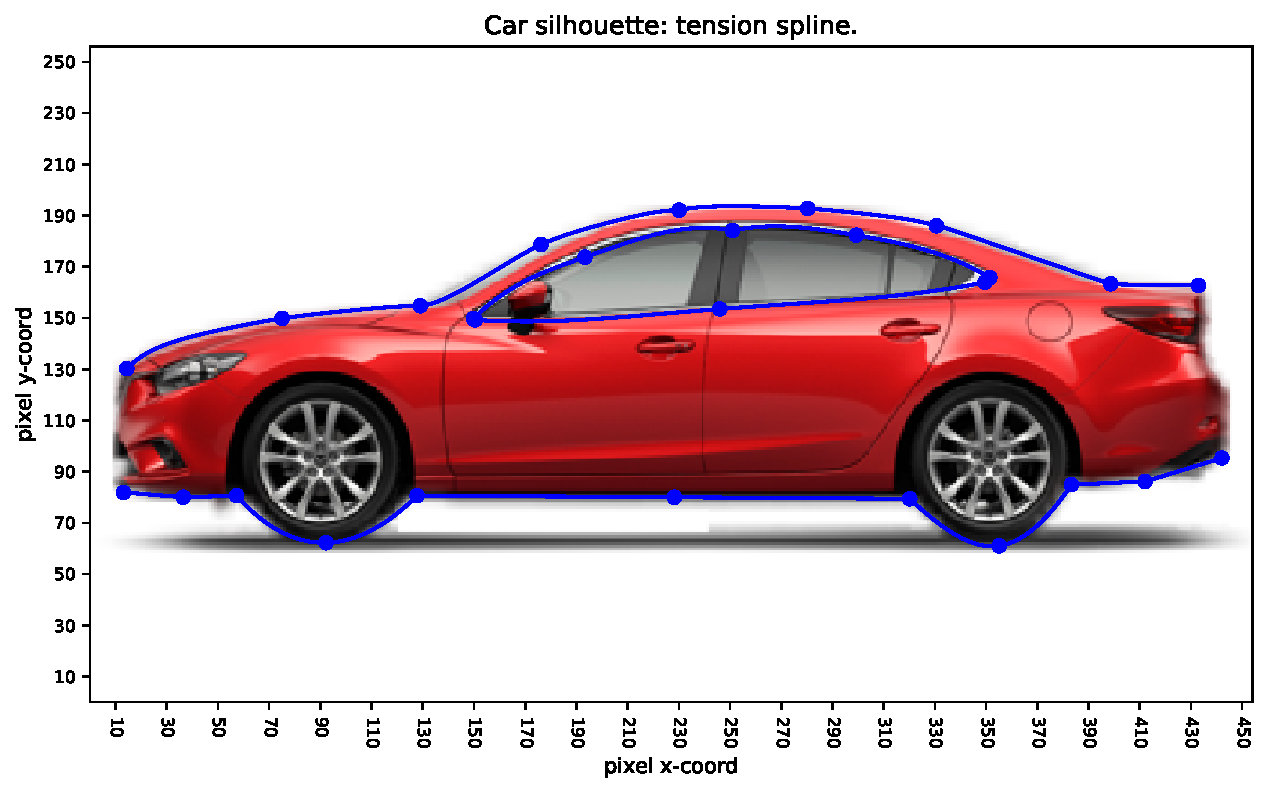
\includegraphics[width=\columnwidth]{figs/p2-car-tension-splines-extra-large.pdf}
  \caption{Larger version of fully splined car.}
\end{sidewaysfigure}


%\verbatiminput{data/points.txt}


\end{document}
